%authors:  coordinated by M. Maggiore and C. van den Broeck, from individual  contributions by  N. Bartolo, E. Belgacem, D. Bertacca, M.A. Bizouard, M. Branchesi, S. Foffa, J. Garcia-Bellido, T. Hinderer, M. Maggiore, S. Matarrese, C. Palomba, M. Peloso, A. Ricciardone, M. Sakellariadou and C. van den Broeck. 
\chapter{Science Case}
\label{chap:ScienceCase}

The gravitational-wave (GW) detectors of second generation (2G), Advanced LIGO and Advanced Virgo, have truly opened a new window on the Universe. The first direct detection of GWs from a binary black hole (BH) coalescence, in September~2015,  was a historic moment, and the culmination of decades of efforts from a large community. Another historic moment was the first detection of a neutron star (NS) binary coalescence, together with the simultaneous detection of the associated gamma-ray burst, and the subsequent observation of the electromagnetic counterpart in all bands of the electromagnetic spectrum. A number of additional detections have taken place since,  to the extent that, at the current level of sensitivity of 2G experiments, BH-BH detections are taking place on a weekly basis.
Many remarkable results in astrophysics and in fundamental physics have already been obtained thanks to these first detections. To mention only a few highlights,  the observation of the NS-NS binary coalescence GW170817 solved the long-standing problem of the origin of (at least some) short gamma ray bursts; the multi-band observations of the associated kilonova revealed that NS-NS mergers are a site for  the  formation of some of the heaviest elements through r-process nucleosynthesis; the observation of tens of BH-BH coalescences has  revealed a previously unknown population of stellar-mass BHs, much heavier than those detected through the observation of X-ray binaries, and has shown that BH-BH binaries exist, and coalesce within a Hubble time at a detectable rate.  Concerning  fundamental physics, cosmology and General Relativity (GR), the observation of the GWs and the gamma-ray burst from the NS-NS binary GW170817 proved that the speed of GWs is the same as the speed of light to about a part in $10^{15}$; the GW signal, together with the electromagnetic determination of the redshift of the source, provided the first measurement of the Hubble constant with GWs;  the tail of the waveform of the first observed event, GW150914, showed  oscillations consistent with the prediction from General Relativity  from the quasi-normal modes of the final BH; several  possible deviations from GR (graviton mass, post-Newtonian coefficients, modified dispersion relations, etc.) could be tested and bounded.

Extraordinary as they are, these results can however be considered only as a first step toward our exploration of the Universe with GWs.
Third-generation (3G) GW detectors, like the Einstein Telescope (ET), will bring the  gravitational wave astronomy revolution to a full realisation. Thanks to an order of magnitude better sensitivity and a wider accessible frequency band with respect to second-generation detectors, 3G detectors will allow us to address a huge number of key issues related to  astrophysics, fundamental physics  and cosmology. 
An example of   the extraordinary potential of 3G detectors is provided  by Fig.~\ref{fig:gw_horizons}. The figure shows the detector reach, in term of cosmological redshift, as a function of the total mass of a coalescing binary. We see that the coalescence of  compact binaries with total mass  $(20-100)~\Msun$, as typical of BH-BH or BH-NS binaries, will be visible by ET up to redshift $z\sim 20$ and higher, probing the dark era of the Universe preceding the birth of the first stars. (In particular, BH-BH mergers seen at such distances would necessarily have a primordial origin.)
By comparison, in the catalog of  detections from the O1 and O2 Advanced LIGO/Virgo runs, the farthest BH-BH event is at $z\simeq 0.5$ and, at final target sensitivity, 2G detectors should reach $z\simeq 1$. The range of BH masses accessible will also greatly increase; as we see from  Fig.~\ref{fig:gw_horizons}, ET will be able to detect BHs with masses up to several times $10^3~\Msun$, out to $z\sim 1-5$.

\begin{figure}[t]
 \centering
 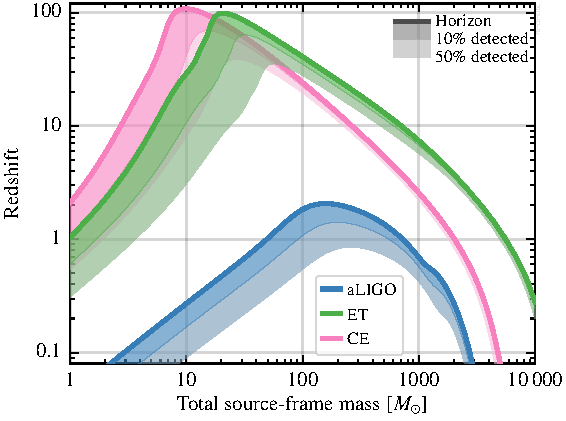
\includegraphics[width=0.6\textwidth]{Figures/gw_horizons_reduce.pdf}\qquad\qquad
% \hspace{-0.09\textwidth}
%  \includegraphics[width=0.4\textwidth]{Figures/waterfall_ET+2CE_maxspin0_q1.pdf}
 \caption{\small Astrophysical reach  for equal-mass, nonspinning binaries  for Advanced LIGO, Einstein Telescope and Cosmic Explorer. 
%Right: lines of constant signal-to-noise ratio in the  (total mass, redshift)  plane, for a network of one ET and two CE detectors. The curves shown assume equal-mass binary components.
}
\label{fig:gw_horizons}
\end{figure}


For NS-NS binaries, whose  total mass is around $3\,\Msun$,  ET will reach $z\simeq 2-3$; by comparison, the NS-NS binary GW170817 was at $z\simeq 0.01$ and, at final target sensitivity, 2G detectors should reach $z\simeq 0.2$.
The corresponding detection rates will be impressive, of order 
$O(10^6)$ BH-BH and $O(10^5)$ NS-NS
%$10^5-10^6$ BH-BH and NS-NS 
coalescences per year; depending on the network of electromagnetic
facilities operating at the time of 3G detectors, over a few years one might
collect $O(10^2-10^3)$     NS-NS GW events with  observed electromagnetic
counterpart. The signal-to-noise ratio of many of these events will be huge,
even for events at cosmological distances.


\emph{The combination of distances and masses explored, sheer number of detections, and detections with very high signal-to-noise ratio will provide a wealth of data that have the potential of triggering revolutions in astrophysics, cosmology and fundamental physics.} 


Beside coalescing binary systems, ET will be able to detect several other kinds of signals, such as stochastic backgrounds of GWs, signals from isolated pulsars, or supernovae, with a sensitivity that improves by orders of magnitude compared to 2G detectors.
Many of the possible achievements of ET, and other planned 3G detectors like Cosmic Explorer in the U.S., are only possible through gravitational waves. For others, GW detectors are complementary to  facilities exploiting electromagnetic radiation  or other messengers, such as neutrinos and cosmic rays. The combined observations through GWs, electromagnetic signals, neutrinos and/or cosmic rays, will give us a multi-messenger picture of many phenomena of the Universe.
Schematically, we can identify the following main items as part of the ET science case:

%\vspace{2mm}

\begin{itemize}
\item Astrophysics:
  \begin{itemize}
   \item black hole properties: origin (stellar vs. primordial), evolution, demography;
   \item neutron star properties: interior structure (QCD at ultra-high densities, exotic states of matter), demography;
   \item multi-messenger astronomy: nucleosynthesis, physics of jets, cosmic rays accelerations, role of neutrinos;
   \item detection of new astrophysical sources of GWs: core collapse supernovae, isolated neutron stars, stochastic background of astrophysical origin.
  \end{itemize}
\item Fundamental physics and cosmology:
  \begin{itemize}
   \item the nature of compact objects: near-horizon physics, tests of no-hair theorem, exotic compact objects;
 % \item Tests of  General Relativity (post-Newtonian expansion, strong field regime, no-hair theorem, ...)
  \item dark matter: primordial BHs, axion clouds, dark matter accreting on compact objects;
  \item dark energy and modifications of  gravity on cosmological scales;
   \item stochastic backgrounds of cosmological origin and connections with high-energy physics (inflation, phase transitions, cosmic strings).
  \end{itemize}
\end{itemize}

% \vspace{2mm}\noindent
It should  be stressed, however, that many questions cross the borders between  domains outlined above. For instance, understanding whether the BHs observed by GW detectors are of stellar or primordial origin obviously has an astrophysical interest, but a primordial origin would have deep consequences on  our understanding of early Universe physics, inflation, etc., subjects that belong to the domain of cosmology and of fundamental physics. As another example, determining the equation of state in the core of neutron stars is of great importance both in astrophysics and for understanding the theory of strong interactions, QCD, in the regime of ultra-high  density, where phase transitions can take place.
 
In the following we briefly discuss some of the science that ET will be able to address\footnote{For more
detailed information on the ET science case and full refereences
the reader is referred to M.~Maggiore \textit{et al.}, `Science Case for the Einstein Telescope', \url{https://arxiv.org/abs/1912.02622}.}.

%\cite{Maggiore:2019uih}.

%\section{Astrophysics}\label{sec:astrophy}

\section{Black hole binaries}\label{sect:Blackholebinaries}

Observationally, BHs have been first identified through X-ray binaries - binary systems in which a BH accretes matter from a companion star. The remarkable GW detections of Advanced LIGO/Virgo in the O1 and O2 runs have then revealed a whole new population of stellar-mass binary BHs with much higher masses, $O(20-80) \Msun$.
With BH-BH and BH-NS coalescence, 3G detectors will explore the Universe to
depths that go well beyond  what can be reached by electromagnetic observations
not only of single astrophysical sources, but even of whole
galaxies.\footnote{To understand how this is possible, it is useful to recall
that a BH-BH coalescence such as the first  detected event, GW150914, converted
into GWs an energy of  $3 \Msun c^2$  in just the last few milliseconds of the
coalescence. The peak luminosity of the event,  $3.6\times 10^{56}\, \mathrm{
erg/s}$, or  $200\, \Msun c^2/{\mathrm{s}}$, was an order of magnitude  larger than
the estimated combined electromagnetic luminosity of all star and galaxies in
the observable Universe!} \emph{ET will uncover the  full population of
coalescing stellar and intermediate mass BHs in the Universe, over the whole
epoch since the end of the cosmological dark ages.}
This will allow ET to answer several key questions about the origin and evolution of BH-BH systems. For instance:

%\vspace{1mm}\noindent
(1) The  observations of BH-BH binaries  across the whole epoch of star formation would contain evidence,  accessible in no other way, of the cosmic history of stellar evolution, including the earliest populations of stars formed in the Universe.   

%\vspace{1mm}\noindent
(2) The observations of BH-BH binaries probe the physics of BH formation in situations which lead to mergers.  ET will provide some events with extraordinarily well-measured properties, alongside large samples of mergers from which statistical population characteristics can be extracted.   
   
%\vspace{1mm}\noindent
(3) By comparing the redshift dependence of the BH-BH merger rate with the cosmic star formation rate it will be possible  to disentangle the contribution of BHs of stellar origin from that of  possible BHs of  primordial origin. 
\emph{Showing that at least a fraction of the observed BHs are of primordial origin would be a discovery of fundamental importance not only in astrophysics but also from the point of view of fundamental physics. }

%\vspace{1mm}\noindent
(4) The discovery of luminous quasars at redshift as large as $z\sim 7$ suggests
the existence, at redshifts $z>7$, of a population of `seed' BHs in the range
$(10^2-10^5) \msun$, from which supermassive BHs have grown through gas
accretion.   ET has the sensitivity necessary to detect  BH binary systems
containing  a  BH with mass between  $O(10^2)\,   \Msun$ and  a few times
$10^3\,\Msun$. \emph{Discovering BHs in this mass range and understanding their role as seed BHs would provide the key to understanding stellar and galactic evolution.}

   
\section{Neutron stars} 

%cold, dense matter and NSs
Neutron stars  are extraordinary laboratories for studying the fundamental properties of matter under conditions far from the realm accessible to experiments and first-principles theoretical calculations. In NSs, intense gravity compresses matter to several times the density of an atomic nucleus. Predicting the composition of such matter and the multi-body interactions that provide the pressure to prevent collapse to a BH requires large extrapolations from known physics, and has been a longstanding scientific frontier.   Neutron stars  provide a unique window onto the behavior of QCD, the fundamental theory of strong interactions, in a regime complementary to the higher temperatures and lower baryon densities accessible in collider experiments that probe the quark-gluon plasma. 

The fundamental properties of NS matter give rise to characteristic imprints in the GW signals from NS, both in  binary coalescences and in the GW signal from individual asymmetric NSs, making GWs unique probes of subatomic physics in unexplored regimes. A 3G GW detector with a high sensitivity and large frequency bandwidth such as ET will be critical to shed light on important fundamental physics questions. 
%In particular:

%\begin{figure}[t]
% \centering
% \includegraphics[width=0.40\textwidth]{Figures/NS_Pie.pdf}\qquad\qquad
%  \includegraphics[width=0.48\textwidth]{Figures/phase_diagram.pdf}
% \caption{\emph{Left}: Conjectured interior structure of a neutron star.  \emph{Right}:
%Matter encountered in neutron stars and binary mergers explores a large part of the QCD phase diagram in regimes that are inaccessible to terrestrial collider experiments. (credit: Sanjay Reddy)}
%\label{fig:NSs}
%\end{figure}

\subsection{Coalescing neutron star binaries} 

With 2G detectors, the first observed NS-NS coalescence
GW170817 demonstrated that useful limits on the NSs' tidal deformability, a characteristic parameter that depends on the properties of matter in their interiors, could be extracted from the inspiral part of the GW signal.%~\cite{TheLIGOScientific:2017qsa}. 
However, despite the proximity of GW170817, the inferred constraints on the equation of state of NS matter~\cite{Abbott:2018exr}
are too weak to discriminate between all realistic models, nor do they offer 
new insights about the possibility of phase transitions (e.g. to a deconfined quark phase) in the inner core.
%~\cite{Hebeler:2010jx,Gandolfi:2011xu,Tews:2018kmu}. 
To determine in detail the nature of matter and interactions in NS interiors requires measuring tidal deformability with an order of magnitude higher accuracy. In addition, such high-fidelity measurements must be obtained for a population of NSs spanning a wide range of masses to map out the parameter dependencies and identify potential signatures of phase transitions. Both can be achieved with ET, which will detect a huge number of NS-NS and NS-BH coalescences per year as quantified above, and will observe their signal with up to tenfold higher accuracy. 

A further unique capability of 3G detectors such as ET is the possibility of exploring in detail the signal after the inspiral part of the coalescence, which, for NS-NS binaries, is at frequencies too high for 2G detectors, but will be within the bandwidth of ET for NS-NS binaries within a few hundreds of Mpc. Witnessing the tidal disruption of a NS  will yield further insights into the properties of NS matter under extreme gravity, and tracking the violent collision of two NSs and its aftermath will provide an exceptional window onto fundamental properties of matter in a completely unexplored regime, at higher temperatures and yet greater densities than encountered in individual NSs. 

The coalescence events of NS-NS and NS-BH systems also have key significance as the principal production site of elements heavier than iron in the cosmos. Heavy elements can be synthesized from the neutron-rich material expelled during the merger or tidal disruption of NSs or through winds from the remnant accretion disk. The subsequent radioactive decay of the freshly synthesized elements leads to an electromagnetic transient known as a kilonova. Multi-messenger observations of a large sample of NS-NS binaries will provide the unique opportunity to study heavy element formation at its production site, to determine how the initial conditions of an astrophysical binary system map to the final nucleosynthetic yields, and the extent to which different NS-NS binary progenitors contribute to the cosmic abundances over time.

\subsection{Continuous waves from spinning neutron stars}

A spinning NS, isolated or in a binary system, if asymmetric with respect to its rotational axis, can also emit continuous semi-periodic GWs. Such asymmetry can derive from frozen deformations produced right after its violent birth, from a strong enough inner magnetic field, or from non-axisymmetric motions or density perturbations. 
No continuous gravitational wave signal has so far been observed  by Advanced LIGO/Virgo.
\emph{The detection of continuous GWs from NS by ET would be a fundamental breakthrough, that would provide   clues about  the condition of formation of isolated NS,  their spin, thermal evolution and magnetic field. Furthermore,  observing such signals with ET's exquisite sensitivity would again give information on the inner structure of NS and on the corresponding aspects of nuclear and particle physics, such as the existence of exotic matter in the NS core.} 
The maximum degree of deformation that a NS can sustain depends on the equation of state: for standard equations of state the maximum value of the ellipticity is $\epsilon_{max} \sim 10^{-6}$, but for exotic objects, containing hyperons or quark matter, is expected to be much higher, $\epsilon_{max}\sim 10^{-4}-10^{-3}$. In practice, it is difficult to predict the actual deformation of  a specific NS, that can depend on the star's history and could be well below the maximum sustainable value.   ET will be sensitive to ellipticities of the order of few times  $10^{-10}$ for the nearest millisecond pulsars, and of $\sim 10^{-6}-10^{-7}$ for young pulsars. 
 It is quite impressive to realize that detecting GWs due to an eccentricity of, say, $\epsilon=10^{-7}$ in a NS means that we would detect the effect  due to a ``mountain'' on a NS, with a  height of about $10^{-7}\times 10\, \mathrm{km}=1\, \mathrm{mm}$!  %(or $10^{-2}$\,mm, for $\epsilon=10^{-9}$).

The maximum distance at which a continuous wave source would be detected
%,  assuming that the source spin-down is dominated by the emission of GWs and an observation time of a few years, 
depends on both the ellipticity and the rotational frequency of the NS. For instance,  a neutron star spinning  at 50\,Hz (and then emitting a continuous GW signal at 100\,Hz) would be detectable by ET  in the whole Galaxy as long as its ellipticity is larger than $10^{-7}$. 
Very  fast spinning  and highly distorted neutron stars,  such as newborn magnetars produced in core collapses or as post-merger remnants of coalescing binaries, could lead to detectable emission at even higher frequencies. In this case the signal can only be observed for a shorter time, since these objects  
are characterized by a very high spin-down and the signal frequency eventually leaves   the detector sensitivity band within a  few days. However, at birth they could have ellipticities as large as $10^{-3}$ so,  even taking into account uncertainties in the data analysis due to the very large initial parameter space (initial frequency, spin-down, braking index), these objects could still be detected out to distances of  tens of megaparsecs.
 

\section{Multi-messenger astrophysics: synergies with other GW detectors and electromagnetic/neutrino observatories}
\label{sec:MM}
%\newcommand{\TOFIX}[1]{\textcolor{red}{#1}}
%\subsection{Synergies with other GW detectors and multi-messenger astrophysics}


ET, with its triangular configuration corresponding to three nested interferometers, is designed to have an extraordinary science output even when operated as a single GW detector. However, a further enhancement of its capabilities will take place when making use of  the synergies with other detectors that could be operating at the same time.

\subsection{Networks of 3G gravitational-wave detectors}

The first obvious synergy is with other GW detectors of third-generation, like the Cosmic Explorer (CE) under study in the US. The most important improvement of a network of three 3G detectors, compared to a single detector, concerns the accuracy in the localization of the sources. For the continuous GWs emitted by spinning NSs a single ET detector  already provides a very accurate parameter estimation - including position - thanks to the very specific modulation of the signals due to Doppler effect induced by the Earth motion.   For coalescing NS-NS binaries a single ET detector (especially in the ET-D configuration with low frequency cutoff in the sensitivity curve) still has some localization capability since, for a low-mass system such as a binary NS, the signal can stay in the detector bandwidth for a long time,  of order of a few days, and again the modulation due to  the Earth motion allows us to localize the source. In this case  an average angular resolution would be around  $150\deg^2$\, for a binary NS at $z=0.1$, but can become of order of just a few $\deg^2$ for the best localized 
sources.
%~\cite{Zhao:2017cbb,Chan2018}. 
No significant localization will be available for BH-BH and BH-NS binaries, that because of their higher total mass will stay in the detector bandwidth for a much shorter time.
A  network of three GW detectors, in contrast, will have quite  good localization accuracy  for all types of binary coalescences; for example a large fraction of NS-NS binaries will have sky localization smaller than 1 deg$^2$ up to $z=0.5$. 
In terms of science output, this means that a 3G detector network will be able to provide good localization information to electromagnetic telescopes, for the search of electromagnetic counterparts. 
%(in the case of systems involving NS; no electromagnetic counterpart is expected for BH-BH systems). 


On the other hand, the different sensitivity curves planned for  ET and CE imply that, from other points of view, these detectors will be complementary. For instance,  as can be seen from  Fig.~\ref{fig:gw_horizons}, ET will be  able to detect heavier systems, with total masses  higher than $10^3~\Msun$ (thanks to its sensitivity in the low frequency regime), while CE has a greater reach  for light systems such as NS-NS binaries.
The different sensitivity curves also mean that, for a given astrophysical system, the signal-to-noise ratio is accumulated differently in ET and in CE, providing complementary information.



\subsection{Joint gravitational and electromagnetic observations}
\label{sec:MM-EM}

The discovery and electromagnetic follow-up of GW170817 showed the enormous potential  of gravitational-wave observations for multi-messenger astrophysics. The gravitational-wave observations combined with the results from the extensive multi-wavelength observational campaign (still undergoing) had a huge impact on our knowledge of the physics of compact objects, relativistic jets, nucleosynthesis, and cosmology. Identifying the electromagnetic signatures of the gravitational-wave sources enables to maximize the science return from a gravitational-wave detection.  
Several future observatories, with a large involvement of the European community, will have strong synergies with ET. SKA, LSST, the THESEUS mission concept, and CTA will be able to observe large regions of the sky from the radio, optical to the X-ray and very high energy, going to deeper sensitivity than current observatories; a 40-meter class telescope such as ELT and a satellite like ATHENA will be able to characterize the source in the optical and X-ray band respectively. 

The ET lower frequency capability enables 
the accumulation of a significant signal-to-noise ratio before the merger, making possible an early detection and warning for the electromagnetic/neutrino followup. Requiring a signal-to-noise ratio of $\geq\,12$ and a sky localization smaller than 100\,deg$^2$, ET can send an early warning alert between 1 and 20 hours before the merger (with the mean of the distribution at about 5\,hours) for signals at 40\,Mpc. 
%\cite{Chan2018}. 
At 200\,Mpc, about 30\% of the detectable signals would accumulate enough SNR for early warning between 1 to 6 hours prior to the merger; about 10\% of the detectable sources within 400\,Mpc can still be announced with an early warning smaller than 1\,hour. This enables the detection of early electromagnetic emission, which is fundamental to understand the physics of the engine and the merger remnant.



%\subsubsection{Nucleosythesis and kilonova emission}
%The cosmic origin of elements heavier than iron has long been a mystery. The thermal emission in the ultraviolet, optical, and near-infrared detected with GW17017 is consistent with kilonova emission powered by the radioactive decay of  heavy nuclei synthesized in the merger ejected by the rapid neutron capture process (r-process). The kilonova associated with GW17017 provided the first observational test to theoretical models which predict r-process nucleosynthesis during  binary neutron star mergers. Spectra, emission timescale and color evolution are directly related with the amount of mass ejected during and after the merger, the ejected mass, velocity, the opacity of the sythetized elements, and the merger remnant. In contrast with supernovae, the spectra do not show narrow lines, but results in an initial featureless smooth optical spectrum due to the blending of lines coming from the high expansion speed of the photosphere, followed by broad absorption features in the near infrared due to lanthanide nuclei synthesized in the merger ejecta. On the basis of the merger rate estimated using the LIGO and Virgo observations and the amount of ejected mass estimated by the kilonova observations, binary neutron star mergers are now understood to be a major channel of r-process production, able to explain the r-process abundances in the Milky Way stellar population. However, it is still uncertain the role of rare classes of supernovae, such as the collapsars associated with long gamma ray bursts, which are expected to be an additional significant source of r-process elements \cite{Siegel2019}. Only a larger sample of kilonova, possibly extending to larger distance, will enable to probe the details of the kilonova emission mechanism, the role of the neutron/black hole merger, and the formation of heavy elements along the cosmic history. 
%
%When ET is expected to observe the sky, LSST will operate as a wide field-of-view survey able to detect kilonova emission up to 800 Mpc. Up to the same distance photometric and spectroscopic characterization will be possible using ground-based 30--40 m telescopes such as TMT and ELT, and the space telescope JWST.  The binary neutron star mergers detectable in this volume are order $10^3$ per year;  for a large fraction of these sources the error box in the  gravitational-wave localization at a distance $> 400$ Mpc  will make  difficult to identify the optical counterpart  among many optical transient contaminants. Still, a significant number of joint GW/electromagnetic detections are expected, in particular if there will  be a detection with an accurate sky localization at high-energy (see the following subsection). For joint gravitational wave/kilonova detection, the precision of parameter estimation for the progenitor system (total mass, mass ratio, spin, and neutron star tidal deformability) and the detection of the signal from the merger remnant made possible by ET represent an unprecedented opportunity to understand the physics governing the kilonova emission, and the nature and equation of state of neutron stars.

%\subsubsection{Relativistic astrophysics and short gamma-ray bursts}

A single ET detector, even in the absence of good source localization, will still be able to perform joint observations with gamma-ray burst (GRB) detectors, through  the observation of a temporally coincident GRB. In turn, this  can  allow for the measurement of the redshift of the source when the high-energy satellite is capable to precisely  localize it. Indeed, GRB satellites such as "Swift" regularly alert ground based spectrographs to obtain the redshifts of the host galaxies of the detected GRBs. 

%Approximately two seconds after GW170817, the Fermi space telescope detected a weak short-duration gamma-ray burst, GRB170817A. Even if it showed the classical observational features that led to classify it as a short GRB, its total gamma-ray energy of about $10^{46}$ erg was many orders of magnitude smaller than the typical energy of any GRB observed before. Nine and sixteen days after the  GW observation of the merger, X-ray and radio emissions were also detected. Over longer timescale the radio, optical, and X-ray observations showed a slow achromatic flux increase until about 150 days before starting to decline. High-resolution radio observations were able to constrain the source size and to show a source displacement consistent with the launch of a jet which successfully breaks through the ejecta developing an angular structure; a narrow ultra-relativistic jet surrounded by less-collimated and slower material. The  structured jet was observed off-axis (i.e. the observer was misaligned with respect to the collimated ultra-relativistic jet). However, while multi-wavelength observations over two years have built a broad consensus about the interpretation of the non-thermal afterglow emission, the origin of the extremely faint prompt gamma-ray emission observed far from the jet core is still under debate; a gamma-ray emission arising from the slower part of the jet or a gamma-ray emission due to shock breakout from thermal energy in a cocoon produced by the jet-ejecta interaction.


The discovery of the gamma-ray emission  associated with GW170817 and the following afterglow observations significantly improved our knowledge of short GRB jets. However, only a detector such as ET will provide the unprecedented capability to completely probe short GRB jet properties by exploring up to high redshift a large population of neutron star mergers observed perpendicular to the orbital plane (on-axis) and off-axis. Mission concepts such as THESEUS will be able to detect $20-40$ on-axis short GRB/year with a localization accuracy of $1-5$ arcmin up to a redshift $z\simeq 5$.
%~\cite{Stratta:2017bwq}.  
After each detection, the rapid alert system will enable to point ground-based spectrographs, such as the ones in ELT and satellites such as ATHENA. THESEUS will give the precise position of the source, and ET and the multi-wavelength follow-up will allow us to connect detailed information of the progenitors and merger remnant properties to the jet and environment properties. It will be possible to build a statistical sample of binary neutron star mergers  able to probe the shape of the jet structure, if it is universal, and investigate what is the typical opening angle for short GRBs. It will be possible  to constrain the  luminosity function  of short GRBs and its relation to the jet structure and the intrinsic luminosity evolution, and to understand what is the efficiency of the jet to break through the material surrounding the NS-NS mergers. Finally, we will understand  the role of NS-BH binaries as progenitor of short GRBs. ET will be crucial to identify the nature of the binary neutron star merger remnant (black-hole, unstable or stable neutron star) and how this is connected to the short GRB central engine and afterglow properties.

%ET will guarantee that instruments such as THESEUS will have a gravitational-wave detection for each detected on-axis GRB. Over a few years, it will be possible to build a sample of tens to $O(100)$  joint detections with luminosity distance measured by gravitational-waves and  redshift measured by ground-based telescopes, such as VLT and ELT. These detections will provide precise measurements of the Hubble constant, helping to break the degeneracies in determining other cosmological parameters obtained by CMB, SNIa and BAO surveys, and to study the nature of dark energy~\cite{Belgacem:2019tbw};  see section~\ref{sec:cosmos} for details.
%
%The detection of a faint off-axis gamma-ray signal such as the one observed by Fermi and INTEGRAL for GW170817, will be difficult for present and the planned future detectors at distances larger than 100 Mpc. However, a fraction of NS-NS merger are expected to produce long-lived neutron stars. In this case, soft X-ray transient can be powered by the new-born neutron star spin-down emission. Even if never observed so far, this emission is expected to be powerful and nearly isotropic \cite{Metzger2014,Siegel2016}. Large field of view instruments, such as the one on board of THESEUS, will allow to detect  the brighter emissions up to 1 Gpc, thereby increasing the numbers of joint GW/electromagnetic detections to a few hundreds per year. 


%\subsubsection{Multi-messenger observations and core collapse supernovae}
%
%Despite the remarkable progress of the theory, the explosion mechanism of supernovae is still an open question, and being able to measure the dynamics of matter at the onset of the phenomena would bring invaluable information to the understanding of the physics of gravitational core collapse. 
%What is fairly known since the 1970's is the role of the neutrinos in the explosion mechanism. During collapse, the stellar core becomes opaque to neutrinos, producing a degenerate sea of trapped neutrinos within it, which subsequently diffuses out of the core on a timescale of order tens of seconds as the nascent proto-neutron star  cools and deleptonizes.
%The three-flavor neutrino flux emanating from the proto-neutron star could power itself a core collapse supernova  via neutrino heating on delayed timescales of order one second. This phenomena is central to most models today, with the exception of models of rare events involving significant rotation, which may be powered magneto-hydrodynamically and where the dynamics proceeds  on shorter timescales. 
%
%Core collapse SNe are not a guaranteed source for ET. A general consensus from all modern numerical simulations is that the expected GW signal is weak (GW released energy of the order of $10^{-9}$~$M_\odot c^2$). Furthermore, the likely diversity of the GW emission mechanisms that are at play in SN explosion makes quite difficult to use matched filtering techniques for digging the signal out of the noise, contrary to what can be done with coalescing binaries or spinning neutron stars. As a consequence,
%the detection of a core collapse supernova GW signal is very challenging
%and the discovery horizon of the current 2G detectors is limited to our galaxy. The expected galactic rate of type II/Ib supernova is also rather small (~1 per 30 years). ET will extend the reach to our galactic neighborhood, so that the expected rate is such that, while detection is not assured, still it is a realistic possibility.  
%
%However, a detection of the GWs emitted in core collapse would be a milestone, revealing the inner mechanisms of core collapse and opening remarkable perspectives  in multi-messenger astronomy. In particular,
%the neutrino emission which will be in coincidence with the GW emission, within few milliseconds, should be detected by the current and future low energy neutrinos detectors (Super-K/Hyper-K, DUNE, JUNO, IceCube, the LVD, Borexino and KamLAND) with a higher signal to noise ratio than the GW signal and a very precise time resolution (few milliseconds) which is a fundamental information to search for a  signal with low 
%signal-to-noise ratio  in the GW data. The false alarm rate of GW searches can be significantly improved with the temporal localization given by the neutrino signal. Furthermore, there exists a strong correlation between the GW and neutrino signals as they are produced at the same interior location and will be powered by the downward accretion plumes associated with hydrodynamic instabilities present in the post-shock flow. These plumes and instabilities will modulate both signals.
%If the signal is likely to remain short (of the order of 1~s), it is expected to be wide band (from few Hz up to several kHz), with very different mechanism in each frequency band. The low frequency and high frequency ET conception design is very well suited for detecting such kind of GW signal.
%
% 

\subsection{Neutrinos and cosmic rays}

Shock-accelerated particles (protons and nuclei) interacting with matter and photons produce neutrinos. The astrophysical sources of gravitational-wave transient signals associated with gamma-ray bursts (GRBs), soft gamma-ray repeaters (SGRs), and core-collapse supernovae are expected to emit neutrinos. While gravitational waves produced by the bulk motion of matter carry information on the astrophysical source dynamics, neutrinos give direct information on interactions between accelerated particles with matter and radiation surrounding the sources. GWs and neutrinos probe the innermost regions of the source typically opaque to the electromagnetic emission. GRBs and SGRs are expected to emit high energy cosmic neutrinos (HEN) from MeV to PeV. In the GRBs, TeV-PeV HENs are expected to be produced in the baryon-loaded jets during the prompt gamma-ray emission, and PeV-EeV HENs during the afterglow phase. In SGRs, the HEN production is expected from protons accelerated by the sudden magnetic reconfiguration. 

When ET will be operational, the upcoming multi-cubic-kilometer neutrino detector KM3NET, and the 10\,km$^3$ facility in the Southern hemisphere IceCube-Gen2 are expected to observe the sky. The sensitivity of the neutrino detectors will make the simultaneous detection of neutrinos and GWs from on-axis short GRBs possible. The high-energy neutrinos would serve as a powerful probe of cosmic-ray acceleration in GRBs and of the physics of relativistic jets associated with NS–NS and NS-BH mergers. For long GRBs and SGRs, the joint detection is less likely and more uncertain. Some models predict that GRBs produce Ultra-High Energy Cosmic Rays (UHECR). In the case of cosmic ray, the astrophysical source identification is complicated by the cosmic ray deflection and the time delay between the arrival of cosmic rays and photons, GW and neutrinos imparted by magnetic fields in the galaxy hosting the source, our Galaxy, and in the intergalactic medium. In this context, ET together with gamma-ray observatories, such as Fermi, HESS, MAGIC, VERITAS, Fermi, CTA and neutrino detectors will make it possible to probe the GRB population, their progenitors, and the jet properties and composition. This will be crucial to probe the role of GRBs as possible sources of UHCRs.

Core-collapse supernovae emit low-energy neutrinos, as proved on February 23, 1987, when neutrinos with energies of a few tens of MeV emitted by the supernova SN1987A, exploded in the nearby Large Magellanic Cloud, were recorded simultaneously by the Kamiokande-II, IMB, and Baksan detectors a few hours before its optical counterpart was discovered. Simultaneous detection of GWs and neutrinos from core collapse of massive star would open remarkable perspectives in multi-messenger astronomy. They are unique probes to reveal the inner mechanisms of the explosion, the dynamics of the remnant (possible a newborn neutron star) and the physics of the post-shock region. The current and future low-energy neutrino detectors Super-K/Hyper-K, DUNE, JUNO, IceCube, the LVD, Borexino, SNO+ and KamLAND are expected to detect neutrinos from the core-collapse SNe, whose GW signal will be detectable by ET. The very short time delay among GW emission and neutrinos (expected to be less than a few milliseconds) represents also a fundamental information to search for signals with low signal-to-noise ratio in the GW/neutrino data.

\subsection{Multi-band GW observations with LISA}

Another potential very interesting synergy could take place with the space interferometer LISA, should ET be operational  by the time that LISA will take data (launch scheduled for 2034, operational from 2036 for a nominal duration of four years), or up to a few years  after the end of the mission. This would allow multi-band GW observations, i.e. the observation of GW signals in widely different frequency bands. In particular, from the rate of BH coalescences inferred by the Advanced LIGO/Virgo O1 and O2 runs, 
we expect that LISA, in a 4\,yr mission, will detect several tens of stellar-mass BH-BH binaries.
%we know that  LISA will detect at least $O(100)$ stellar-mass BH-BH  binaries during their inspiral phase, up to $z\simeq 0.4$.
%~\cite{Audley:2017drz}.   
Months to years later, several of these events will cross into the ET window, where they will coalesce. For instance, the first observed GW event, GW150914,  
would have been detected by LISA a few years before coalescence,
%~\cite{Sesana:2016ljz}, 
if  at that time LISA had already been  in orbit.


Multi-band observations would have many benefits: a joint LISA-ET detection would provide
sky localization of the source with an error of only a few square degrees, and 
would make it possible to alert telescopes and look for an electromagnetic counterpart, both  in the pre-merger and post-merger phases (which in principle is not expected for BH-BH coalescences, but could be present in BH-NS binaries); it
would improve parameter estimation, reducing the error on the luminosity distance to the source and on the initial spins  and  allowing to measure with extreme precision the sky position, mass and spin of the final BH. LISA and ET observations of such events would be highly complementary; for instance LISA, by observing the long inspiral phase, will measure very accurately the masses of the initial BHs, while ET  would detect  the last few cycles and the merger, and would therefore measure the final masses and spin from the ringdown of the final BH. Consistency tests  between the
inspiral part of the waveform and the merger-ringdown part, of the type performed 
%in \cite{TheLIGOScientific:2016src} 
for the first detection GW150914, would then provide very stringent tests of General Relativity.
%~\cite{Vitale:2016rfr}.
Furthermore, the early warning provided by LISA on particularly interesting events might allow real time optimization of ET  to improve sensitivity to the ringdown signal.
%~\cite{Tso:2018pdv}.

\section{Fundamental physics and cosmology}

The direct detection of gravitational waves has started to give us access to the genuinely
strong-field dynamics of spacetime. This is illustrated in Fig.~\ref{fig:phasediagram}, which shows how 
different kinds of observations (past, current, and future) will give us access to different
regimes, in terms of spacetime curvature $R$ and gravitational potential $\Phi$ (which for binary 
systems can be traded for $v^2/c^2$, where $v$ is the characteristic speed of the binary and $c$
is the speed of light). 

\begin{figure}[t]
\centering
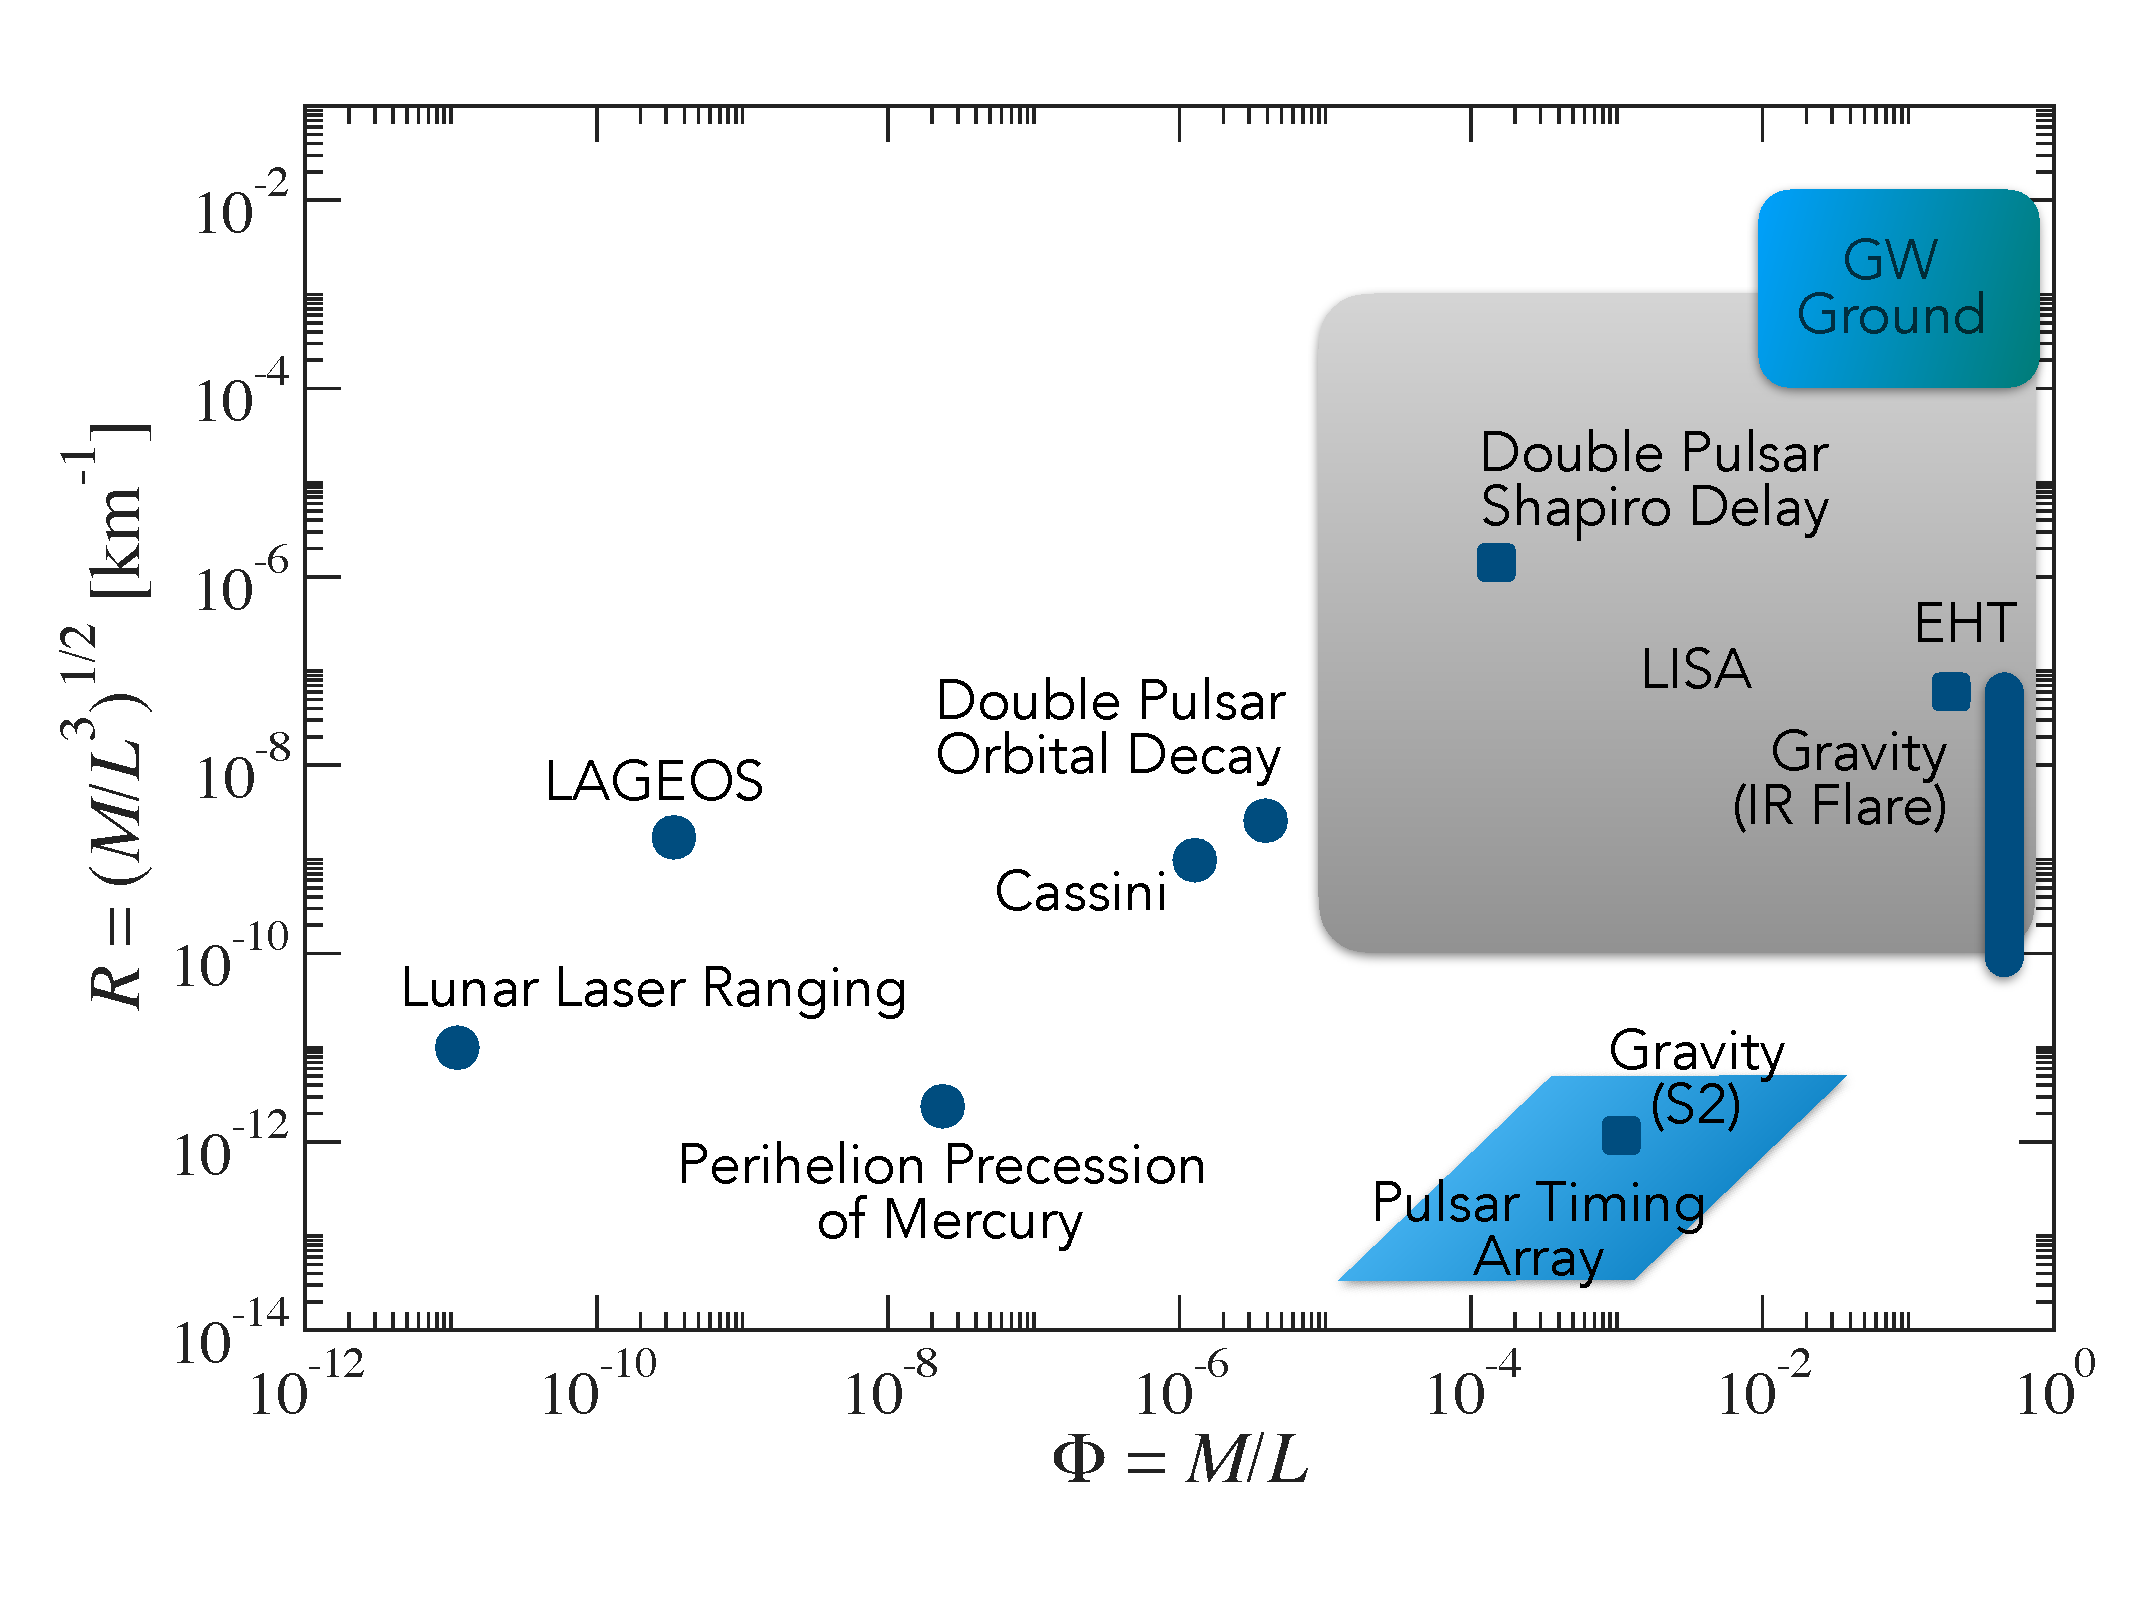
\includegraphics[width=0.8\textwidth]{Figures/ToG2_reduce.pdf}
\caption{\small Probing gravity at all scales: illustration of the reach in spacetime curvature versus potential energy targeted by different  kinds of observations. 
$M$ and $L$ are the characteristic mass and length involved in the system or process being observed. 
The genuinely strong-field dynamics of spacetime manifests itself in the top right of the diagram. The label EHT refers to the Event Horizon Telescope.
Image from the `3G Science Book' by the the GWIC 3G Science Case Team, and the International 3G Science Team Consortium (in preparation, 2020).
%From ref.~\cite{Sathyaprakash:2019yqt}.
}
\label{fig:phasediagram}
\end{figure}

Observations of GWs from binary BH and binary  NS coalescences with Advanced LIGO and Advanced Virgo have enabled us to probe for the first time the regime where both $R$ and $v/c$ are large. By observing the inspiral phase  we could test the predictions of GR (as encoded in the post-Newtonian coefficients) to a precision of about $10\%$.
By observing the full  inspiral-merger-ringdown process of binary black holes, we could perform a first study of the dynamics of vacuum spacetime. 
The observation of the binary neutron star inspiral GW170817 also gave us our empirical 
access to the interaction of spacetime with high-density matter. Because of the large 
distances that GWs have to travel from source to observer, we were able to
strongly constrain possible dispersion that might occur; the latter led to a bound on 
the mass of the graviton of $m_g \leq 5 \times 10^{-23}\,\mbox{eV}/c^2$. These examples
notwithstanding, on the whole the existing detectors lack the sensitivity to put very strong
constraints on possible deviations from Einstein's theory, particularly regarding 
the strong-field dynamics at the source, corresponding to the top right edge of 
Fig.~\ref{fig:phasediagram}. 
The situation will be quite different with Einstein Telescope. One reason is the much 
larger detection rate; especially for the purposes of fundamental physics, information 
from multiple sources can often be combined, and the measurement accuracy on 
common observables  
tends to improve with the square root of the number of detections. 
For example, the post-Newtonian coefficients that govern binary inspiral will be determined with sub-percent to sub-permille accuracy.
However, the fact that
the same GW source will be much louder in ET will also give us access to 
qualitatively new effects. Below we discuss in turn capabilities of ET in 
probing the properties of gravity, as well as unraveling the nature of ultra-compact
objects, with potentially game-changing implications for our understanding of black holes, 
the make-up of dark matter, dark energy, and maybe even quantum gravity itself.



\subsection{Physics near the black hole horizon}%: from tests of GR to quantum gravity}



%\vspace{2mm}
%\noindent
\emph{Testing the GR predictions for space-time dynamics near the horizon}.
Black holes are one of the most extraordinary predictions of General Relativity. They are identified through  their most striking property: in the case of stellar mass black holes, a mass $O(10-100)\,\Msun$ is concentrated in an extremely small volume; for instance, the Schwarzschild radius of a non-rotating BH with mass $10\msun$ is about 30\,km. However, how certain can we be that the massive compact objects that we saw merge with 2G detectors are really the standard black holes of classical General Relativity?

\begin{figure}[t]
\centering
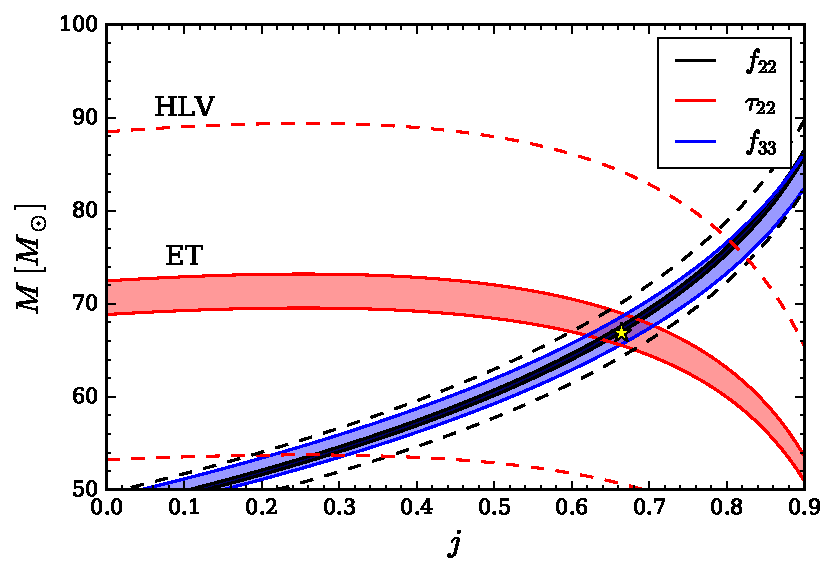
\includegraphics[width=0.7\textwidth]{Figures/3g_ringdown.pdf}
\caption{\small Testing the nature of black holes by using two quasi-normal modes and checking
that the characteristic frequencies $f_{22}$ and $f_{33}$ and the damping time $\tau_{22}$ are consistent
with each other, given that for ordinary black holes these can only depend on two numbers, namely
the final mass $M$ and final spin $j$. The estimates are for the ``ringdown" of the remnant
black hole arising from a binary similar to the source of GW150914. The dashed curves marked HLV 
are the 95\% confidence regions one would obtain from Advanced LIGO-Virgo, while the colored bands
are for ET. The star indicates the true values of $M$ and $j$.
}
\label{fig:ringdown}
\end{figure} 

General Relativity gives detailed and specific predictions on the nature of BHs that a 3G detector such as ET will be able to test. The celebrated no-hair theorem  of GR states that, in  a stationary situation, a BH is determined
by just two numbers: its mass and its spin (plus the electric charge, which however is not relevant in an astrophysical context, where it is quickly neutralized). However, when a BH is perturbed, it reacts in a very specific manner, relaxing to its stationary configuration by oscillating in a superposition of 
quasi-normal modes, which are damped by the emission of GWs. The fact that an elastic body has normal modes is a familiar notion from elementary mechanics. It is however quite fascinating to realize  that a BH, which is a pure space-time configuration, also has its quasi-normal modes. These represent pure space-time oscillations, in a regime of strong gravity, and, in a sense, describe the elasticity of space-time in a most extreme situation, in the region close to the BH horizon. The theory of BH quasi-normal modes is a classic chapter of GR,
%(see \cite{Berti:2009kk,Maggiore:2018zz} for reviews), 
and in particular predicts the spectrum of frequencies and damping times of the quasi-normal modes as a function of the mass and spin of the BH. Highly perturbed black holes arise as the 
remnants of binary BH or NS mergers, and relax to the final stationary BH configuration through GW emission in the quasi-normal modes, in the so-called `ringdown' phase of the coalescence, where the waveform is given by a superposition of damped sinusoids. Indeed, for the first observed BH-BH coalescence, GW150914, the final ringdown phase was just discernable, and was shown to be broadly consistent with the prediction of GR for the value of the parameters inferred from  the inspiral part of the waveform.
%~\cite{TheLIGOScientific:2016src}. 
Fig.~\ref{fig:ringdown} illustrates the difference in the accuracy of such a test between 2G and 3G detectors, for a single source such as GW150914. Furthermore, 
the accuracy of the measurement scales as $1/\sqrt{N}$, where $N$ is the number of detections;
as we saw, ET will detect $N\sim O(10^5-10^6)$ BH binaries, compared to several hundreds expected for 2G detectors.


%\vspace{1mm}
%\noindent 
\emph{Exploring the possibility of exotic compact objects}.
The observation of quasi-normal modes, besides providing a spectacular test of GR in the strong-field, near-horizon regime, could also potentially lead to the discovery of different types of compact objects.
Indeed, various exotic compact objects have been proposed that may act as ``black hole mimickers", such as boson stars, gravastars, etc.
%(see \cite{Cardoso:2019rvt} for review). 
When such  objects are part of a binary system that undergoes
coalescence, they can make their presence known through various possible imprints on 
the GW signal emitted. Already during the inspiral phase, these objects may get tidally deformed in a way that would be impossible 
for a standard, classical black hole. Unlike second generation detectors, ET will for instance be able 
to distinguish neutron stars from boson stars even for the most compact models of the latter.  
Another possibility is that an exotic object could be identified through 
an anomalous spin-induced quadrupole moment, which would again not be accessible with 
current detectors, but measurable with ET to the percent level.
%~\cite{Krishnendu:2017shb}.

If the outcome of a coalescence is different from a BH, this might leave an imprint on  the  ringdown phase, and could be tested by measuring quasi-normal mode frequencies and life-times, as in Fig.~\ref{fig:ringdown}. For exotic compact objects where the modifications take place only at  scales much shorter than the so-called light-ring (as in the case of quantum gravity effects discussed below), the ringdown signal will be very similar to a BH, but after the ringdown has died down, exotic compact objects may continue to 
emit bursts of gravitational waves at regular time intervals, called \emph{echoes}.
%~\cite{Cardoso:2016rao,Cardoso:2017cqb}. 

%\vspace{2mm}
%\noindent
\emph{Signals from quantum gravity?}
Prompted by Hawking's 
information paradox, modifications of the structure of space-time at the horizon scale have been proposed, such as firewalls~\cite{Almheiri:2012rt} and fuzzballs,
%~\cite{Mathur:2005zp}, 
for which the classical horizon is removed through macroscopic quantum effects. 
From a particle physics perspective, one is used to the fact that, at energies $E$ much below the Planck energy scale $M_{\mathrm{Pl}}$, quantum gravity effects are suppressed by powers of 
$E/M_{\mathrm{Pl}}$, and therefore, given that  the Planck scale $M_{\mathrm{Pl}}$ is of order $10^{19}$\,GeV, they are totally unaccessible at accelerators, even in any foreseeable future. Equivalently, at a macroscopic length-scale $L$, quantum gravity effects are suppressed by powers of $l_{\mathrm{Pl}}/L$, where $l_{\mathrm{Pl}}\sim 10^{-35}$\,m is the Planck length. In contrast, near the BH horizon, where the characteristic length-scale $L$ is given by the Schwarzschild radius $R_S$, effects due to quantum gravity  are governed  by a factor  $\log (l_{\mathrm{Pl}}/R_S)$, and can manifest themselves  through a series of echos after the initial ringdown signal,
%~\cite{Cardoso:2016rao,Cardoso:2016oxy,Cardoso:2019apo}, 
emitted with a time delay  $\tau_{\mathrm{echo}}\simeq (R_S/c) \log (R_S/l_{\mathrm{Pl}})$. For instance, for a final object with mass $M=60\Msun$, one has 
$\tau_{\mathrm{echo}}\simeq 16 \tau_{\mathrm{BH}}$, where $\tau_{\mathrm{BH}}\simeq 3$\,ms is the fundamental damping time of a Schwarzschild BH with this mass. Such signals 
 are potentially within the reach of ET, which raises the tantalizing possibility of accessing 
quantum gravity effects at ET.

To summarize, \emph{the transition from second generation observatories to Einstein Telescope
will lead to a qualitative leap in our ability to probe both the nature of gravity in the strong field regime 
and the structure of compact objects, and could even lead to exploring the quantum gravity regime.} 


\subsection{The nature of dark matter}

Understanding the nature of dark matter and of dark energy is one of the crucial problems in astrophysics, cosmology and fundamental physics.  ET will be able to address both questions. 
Observations at ET will allow us to attack the problem of the origin of dark matter from several different angles. Dark matter could be composed, at least in part, of \emph{primordial} black holes in the mass range $\sim 0.1 - 100\,M_\odot$.
%~\cite{Carr:2019hud,Garcia-Bellido:2019vlf,Clesse:2016vqa,Clesse:2016ajp,Garcia-Bellido:2017fdg}. 
Primordial BHs  could be seeded by fluctuations generated during the 
last stages of inflation, which then collapsed in later epochs as a consequence of drops in the pressure of the cosmic fluid, e.g. during the  QCD quark-hadron transition. Their mass distribution depends on the precise model 
of inflation and on the epoch when they  collapsed. The large number of mergers that ET
will see, together with its  ability to access a broad range of masses, would allow us to map the black hole mass distribution
and identify an excess of black holes in certain mass intervals. For black holes with masses well below a 
solar mass, no plausible astrophysical formation mechanism is available, so that their detection would
point to the existence of primordial black holes. A unique advantage of ET is the possibility of observing stellar mass black hole mergers at redshifts of $\sim 10-20$, before any stars had formed that could create black holes in the usual way; 
should such an event be observed then (irrespective of masses) the objects involved are bound to be of primordial origin.

If most of the dark matter occurs in the form of particles beyond the Standard Model, then also in that case gravitational wave observations can be used to search for them. Black holes could not only accrete dark matter particles, but also be subject to gravitational drag, which in a binary system would accumulate over the course of many orbits. 
If ET will be operational during the same period as LISA, joint LISA-ET observations of the same source will then be of great value.
%~\cite{Barausse:2016eii}.
There is also the possibility that dark matter particles are captured in astrophysical objects and thermalize with the star.
%~\cite{Gould:1989gw}. 
The presence of a dark matter core in a neutron star might again have an imprint upon the GW signal during binary inspiral and merger.
In some models,
%~\cite{Bramante:2017ulk,Kouvaris:2018wnh}, 
the accumulation of dark matter may lead to the formation of a black hole inside a neutron star, which then accretes the remaining neutron star matter, leading to black holes of $(1-2) \,M_\odot$ that could be observed by ET.

Finally, ultralight bosons have been proposed in various extensions of the Standard Model, and also as  dark matter candidates.
%~\cite{Essig:2013lka,Hui:2016ltb}. 
If their
Compton wavelength is comparable to the horizon size of a stellar or supermassive 
rotating black hole (\emph{i.e.}~for particle masses of $10^{-21} - 10^{-11}$\,eV),
they can extract rotational kinetic energy from the black hole through ``superradiance" to feed the formation of a bosonic ``cloud" with mass up to $\sim 10$\% of the black hole.
%~\cite{Arvanitaki:2010sy,Brito:2014wla, East:2017ovw}. 
These clouds annihilate over a much longer timescale than their formation, through the emission of nearly monochromatic gravitational waves, which could be detected either directly or as a stochastic background from a large number of such objects throughout the Universe.
Additionally, measuring the distribution of black hole masses and spins can yield an indication of the prevalence of superradiance through light scalars. 
Moreover, the presence of such clouds will again have an effect on binary orbital motion.%~\cite{Baumann:2018vus}. 
In this way GWs have the potential to provide a unique probe into 
an ultralight, weakly coupled regime of particle physics that can not easily be accessed in accelerator experiments.

\emph{To summarize, ET has the potential of discovering several dark-matter candidates that will be inaccessible by any other means.}

     
\subsection{The nature of dark energy}\label{sec:cosmos}

ET will be an outstanding discovery machine for studying the nature of dark energy, using binary NSs and binary BHs as cosmological probes.
Indeed, a remarkable feature of the GWs emitted in the coalescence of compact binaries is that  their signal   provides an absolute measurement of the luminosity distance to the source. The relation between the luminosity distance $d_L$ and redshift $z$ of the source carries crucial cosmological information and is among the main observables of modern cosmology. 

%Observations performed with electromagnetic waves can  infer the redshift of a source,  through spectroscopic or photometric observations; however, obtaining the absolute distance to a source at cosmological distances is much more difficult. Ideally, this requires the existence of a ``standard candle'', a class of sources whose intrinsic luminosity ${\cal L}$ is known, so that, from a measurement of the  energy flux ${\cal F}$  received by the observer, we can reconstruct the luminosity distance $d_L$ from ${\cal F}={\cal L}/(4\pi d_L^2)$.
%A classic example of standard candle in cosmology is provided by type~Ia supernovae: these are bright enough to be visible at cosmological distances, and, after some empirical corrections, their intrinsic luminosity can be considered as fixed; its value is then calibrated through the
% construction of a  ``cosmic distance ladder'', in which classes of sources at shorter distances are used to calibrate different sources at higher and higher distances. Indeed, type Ia Supernovae provided the first conclusive evidence for the  existence of dark energy~\cite{Riess:1998cb,Perlmutter:1998np}, a discovery that was awarded with the 2011 Nobel Prize in Physics.
% 
%GW observations of compact binary coalescences completely bypass the need for empirical corrections and the uncertainties in the  calibration of the cosmic distance ladder, since the observed waveform of the inspiral phase directly carries  the information on the luminosity distance $d_L$~\cite{Schutz:1986gp}. In this context, coalescing binaries are called ``standard sirens'', the GW analogue of standard candles. By contrast, the GW signal does not carry  direct information on the redshift, so the situation is reversed compared to electromagnetic observations. 
%The ideal situation then takes place when one has a joint GW-electromagnetic detection, as was the case for the NS-NS binary GW170817. In this case the GW signal gives $d_L$ and the electromagnetic observation  the redshift $z$. Even in the absence of a redshift determination from an electromagnetic counterpart, several statistical methods have been discussed in the literature, to extract cosmological information from purely GW observations~\cite{Schutz:1986gp,DelPozzo:2011yh,Taylor:2011fs,Taylor:2012db,Messenger:2011gi}.

In the low redshift  limit $z\ll  1$ accessible to 2G detectors, the relation between $d_L$ and $z$ reduces to the Hubble law $d_{L}(z)\simeq H^{-1}_0z$. Hence the observation of standard sirens  at low redshifts can provide  a measurement of  $H_0$. The possibility of measuring $H_0$  has already been demonstrated with  GW170817, from which a value  $H_0=70.0^{+12.0}_{-8.0}\,\mathrm{km}\, \mathrm{s}^{-1}\, \mathrm{Mpc}^{-1}$ was obtained.%~\cite{Abbott:2017xzu}.  
With $O(100)$ standard sirens with counterpart, a measurement of $H_0$ at the $1\%$ level could already be possible with 2G detectors. This would  allow us to  arbitrate the current discrepancy between the  value of the Hubble parameter $H_0$ obtained from  late-Universe probes,
%~\cite{Riess:2019cxk,Wong:2019kwg}, 
and the  value  inferred from early-Universe probes,
%~\cite{Aghanim:2018eyx,Abbott:2018xao}, 
which has currently reached the  $5.3\sigma$ level and can be an indication of deviations from $\Lambda$CDM, the standard cosmological model.


%\begin{figure}[t]
%%\includegraphics[width=0.48\textwidth]{Figures/dgw_su_dem.pdf}\quad\quad
%\centering
%\includegraphics[width=0.4\textwidth]{Figures/xi0_w0.pdf}
%\caption{\small Constraints on the parameters $(\Xi_0,w_0)$  that describe a non-trivial dark energy sector. Modified GW propagation is not accessible by electromagnetic observations from CMB, Baryon Acoustic Oscillations,  and Supernovae, whose contours (red) are flat along the $\Xi_0$ direction. Standard sirens at ET (gray), combined with these electromagnetic probes  allow a determination of $\Xi_0$ 
% to better than $1\%$ (blue). (From ref.~\cite{Belgacem:2018lbp}).
%\label{fig:xi0w0}}
%\end{figure}


With ET, given  the expected huge number of detections and the very high signal-to-noise ratios  of nearby  events, a sub-percent level accuracy on $H_0$  could be reached. However,
a much higher potential for discovery is provided by the fact
that ET will have access to standard sirens at much larger redshifts, where the luminosity distance-redshift relation will be sensitive  to effects  induced by a non-trivial  dark energy  sector and by modifications of General Relativity on cosmological scales. This would allow us to obtain a   measurement of the dark energy equation of state from GW observations.
%~\cite{Sathyaprakash:2009xt,Zhao:2010sz,Belgacem:2018lbp}. 
Actually, the situation for 3G detectors is even more interesting due to a phenomenon of modified GW propagation.  
%(see \cite{Belgacem:2017ihm,Belgacem:2018lbp} and references therein). 
Indeed, in generic theories where dark energy is dynamical and gravity is modified at cosmological scales,  the propagation of GWs over cosmological distances is also modified. 
As a result, the GW amplitude becomes inversely proportional to a ``GW luminosity distance'' $d_L^{\mathrm{gw}}(z)$, different from the standard electromagnetic one $d_L^{\mathrm{em}}(z)$;  the ratio
$d_L^{\mathrm{gw}}(z)/d_L^{\mathrm{em}}(z)$ carries distinctive imprints of the dark-energy sector of the theory. This behavior turns out to be  completely generic to  modified gravity models.%~\cite{Belgacem:2019pkk}. 
For most models, the deviations from GR can be parametrized in terms of two parameters $(\Xi_0,n)$   defined by
$d_L^{\mathrm{gw}}(z)/d_L^{\mathrm{em}}(z)=\Xi_0+(1-\Xi_0)(1+z)^{-n}$.%~\cite{Belgacem:2018lbp}. 
Measuring  modified GW propagation through its effect on the GW luminosity distance is a very powerful probe for the dark energy sector, which cannot be accessed at all with  electromagnetic  observations. With a few hundred standard sirens with counterpart, ET will constrain $\Xi_0$ to below 1\%, a level significantly  smaller than the deviation from GR foreseen by various alternative gravity theories. Indeed, the sector of tensor perturbations over a cosmological background  can only be explored with  GW detectors, and can lead to significant surprises. For instance, one can have a cosmological model that is  observationally indistinguishable from 
$\Lambda$CDM in terms of current electromagnetic observations,
 but still predicts a value of $\Xi_0$  as large as $\Xi_0\simeq 1.8$, representing a $80\%$ deviation from $\Lambda$CDM.%~\cite{Belgacem:2019lwx}.
Such a large effect could be detectable even with just a single standard siren at ET.
\emph{In summary, the sector of cosmological tensor perturbations is  virgin territory that can only be explored by third-generation GW detectors such as ET, and which could  offer the most powerful window for understanding the nature of dark energy and modifications of General Relativity at cosmological scales.}





\subsection{Toward the Big Bang: stochastic backgrounds of GWs}


The weakness of the gravitational interaction, which is responsible for the fact that  GW detection is such a challenging enterprise, 
also implies that the observed GW signals  carry uncorrupted information about their production mechanism. This is particularly significant for stochastic backgrounds of GWs of cosmological origin. For comparison, in the early Universe photons were kept in equilibrium with the primordial plasma by the electromagnetic interaction, and decoupled from it  at a redshift $z\simeq 1090$, when the Universe already had a rather low temperature $T\simeq 0.26$\,eV. The photons that we observe today from the cosmic microwave background  therefore give a snapshot of the Universe at this decoupling epoch, while all information about earlier epochs was obliterated by the photon collisions with the primordial plasma. Neutrinos, which interact through weak interactions, decoupled  when the Universe had a temperature $T\simeq 1$\,MeV.  By contrast, GWs were decoupled from the primordial plasma at all temperatures below the Planck scale $\sim 10^{19}$\,GeV,
corresponding to a far earlier epoch, and energies far exceeding  those accessible to particle accelerators. Gravitational waves from the early times of the universe imprint a signature on the B-mode of the cosmic microwave background, the analysis of which can provide valuable indirect indications of early physical processes. \emph{The direct observation of a stochastic background of gravitational waves of cosmological origin would provide us with an unaltered direct snapshot of the earliest moments after the Big Bang that could not be obtained like this with any other probe.} 
%The difference between these two methods is comparable to the indirect detection of GWs by the Hulse-Taylor pulsar on the one hand and the direct detection of GWs by advanced LIGO on the other.}

In order to detect a stochastic background one has to perform cross-correlation among the outputs of pairs of detectors, as would be possible with a single ET observatory, which is made of three non-parallel detectors.
On the cosmological side, while the background  generated  by the amplification of quantum vacuum fluctuations due to the inflationary expansion is expected to be too low to be detected by  3G detectors, there are several other inflation-related mechanisms that can produce detectable signals.%~\cite{Maggiore:1999vm, Caprini:2018mtu, Maggiore:2018zz}. 
For example,  large GW amplitudes are naturally produced in inflationary models where there are secondary fields coupled to the inflaton.%~\cite{Cook:2011hg,Bartolo:2015qvr}. 
On the other hand, also scenarios alternative to inflation, such as pre-Big-Bang models inspired by string theory,
%~\cite{Brustein:1995ah,Buonanno:1996xc,Gasperini:2002bn}, 
or models where the inflaton is coupled to an axion field,
%~\cite{Domcke:2019zls}, 
predict a spectrum which grows with frequency, resulting in a potentially detectable signal in the ET bandwidth.
Another source of GWs is expected during the preheating period of the Universe, following closely the end of inflation.
%~\cite{Kofman:1994rk,Kofman:1997yn,Greene:1998nh,Greene:2000ew}. 
In particular, when ``preheat'' fields are coupled to the inflaton, these may undergo
a non-perturbative excitation after inflation with the consequent generation of GWs. The amplitude of these backgrounds can be very large, and there are scenarios that can peak at frequencies in the Einstein Telescope range. 
The statistical properties (and, particularly, its deviation from Gaussianity) of the cosmological stochastic GW background will be another possible target for 3G detectors that will allow to distinguish a cosmological background from other stochastic signals.
%\cite{Bartolo:2019oiq}.



First order phase transitions are another potential source of  a stochastic background.
As the Universe expands, its temperature drops and it may undergo a series of phase transitions followed by spontaneous breaking of symmetries. If a phase transition is of first order,  a  stochastic GW background may be produced as true vacuum bubbles collide and convert the entire Universe to the symmetry-broken phase.
In the Standard Model  of particle physics, the electroweak and the QCD  transitions are just  cross-overs, hence any generated gravitational wave signal is not expected to be detectable. However, there are many extensions of the Standard Model (e.g., with additional scalar singlet or doublet, spontaneously broken conformal symmetry, or phase transitions in a hidden sector) which predict strong first-order phase transitions, not necessarily tied to either the electroweak or the QCD phase transition. 

Phase transitions followed by spontaneous breaking of symmetries may leave behind topological defects as relics of the previous more symmetric phase of the Universe.
In the context of Grand Unified Theories,   one-dimensional defects called cosmic strings are generically formed.%~\cite{Jeannerot:2003qv}. 
Cosmic string loops oscillate periodically in time, emitting GWs which depend on a single parameter, the string tension $\mu$, related to the energy scale $\eta$ of the symmetry breaking through $G\mu\sim 10^{-6}(\eta/10^{16}\, \mathrm{GeV})^2$. 
Cosmic strings may also emit bursts of beamed gravitational radiation. The incoherent superposition of these bursts generates a stationary and almost Gaussian stochastic GW background. Occasionally there may also be sharp and high-amplitude bursts of GWs above this stochastic background. 
ET  will be able to improve on 2G bounds on $G\mu$ by up to 8 orders of magnitudes: with just one year of data one can detect or exclude values of $G\mu$ down to  $10^{-17}-10^{-18}$, depending on the loop distribution.
      
%\subsubsection{Astrophysical backgrounds} 
In addition to the cosmological background, an astrophysical contribution will  result from the superposition of a large number of unresolved sources too faint to be detected individually. Examples include short-lived burst sources, such as core collapses to neutron stars  or black holes, oscillation modes of (proto)-neutron stars, or the  final stage of compact binary mergers; periodic long lived sources, typically pulsars; or  the early inspiral phase of compact binaries, whose frequency  evolves  slowly compared to the observation time.%~\cite{Regimbau:2011rp}. 
The strongest astrophysical background in the frequency region of terrestrial detectors is expected to be due to the coalescence of BH-BH and  NS-NS systems.   To separate the cosmological and the astrophysical backgrounds the first step will be to use any distinct spectral dependence of the average (monopole) amplitude $\Omega_{\mathrm{GW}}$.
%~\cite{Caprini:2019pxz}.   
However,  the better angular resolution of 3G detectors will most probably allow us to spot the anisotropies (directionality dependence) of the astrophysical background. Such anisotropies contain information about the angular distribution of the sources and can be used as a tool for source separation as well as a tracer of astrophysical or cosmological structure. The detection of the anisotropies will give the possibility to relate  the properties of GW sources with those of their host galaxies, and in particular their cross-correlation will provide a handle to discriminate the origin of black holes.  On the other hand the effects imprinted in the angular power spectrum of the stochastic background, due to the GW distorsion  by the intervening Large Scale Structure  distribution, like Kaiser, Doppler and gravitational potential effects, can be used to study the Large Scale Structure and  make precision cosmology with 3G detectors.
% \cite{Cusin:2017fwz, Jenkins:2018uac,Bertacca:2019fnt}. 






